% Architecture diagram for CNN-CTC OCR pipeline
% Compile standalone and convert to PDF
\documentclass[tikz,border=5pt]{standalone}
\usepackage{tikz}
\usetikzlibrary{shapes.geometric, arrows.meta, positioning, fit, backgrounds}

\begin{document}
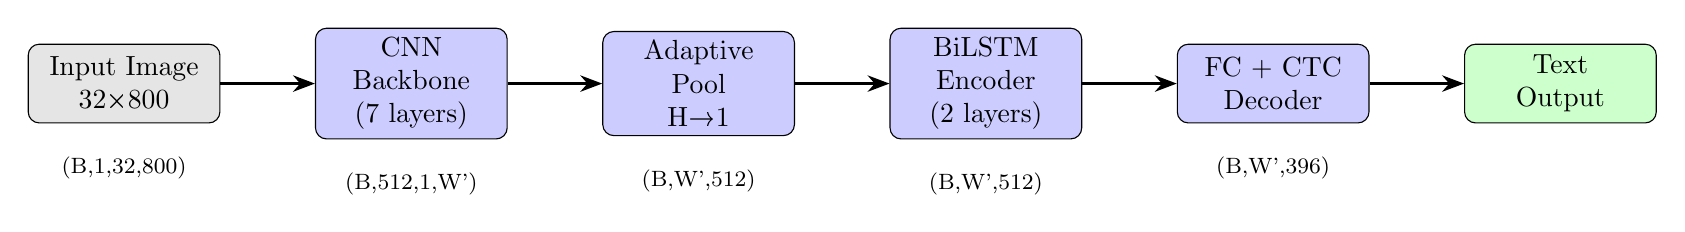
\begin{tikzpicture}[
    node distance=0.8cm and 1.2cm,
    block/.style={rectangle, draw, fill=blue!20, text width=2.2cm, text centered, minimum height=1cm, rounded corners},
    arrow/.style={-{Stealth[scale=1.2]}, thick},
    label/.style={font=\footnotesize, text centered}
]

% Input
\node[block, fill=gray!20] (input) {Input Image\\32×800};

% CNN Backbone
\node[block, right=of input] (cnn) {CNN\\Backbone\\(7 layers)};

% Pool
\node[block, right=of cnn] (pool) {Adaptive\\Pool\\H→1};

% LSTM
\node[block, right=of pool] (lstm) {BiLSTM\\Encoder\\(2 layers)};

% FC + CTC
\node[block, right=of lstm] (ctc) {FC + CTC\\Decoder};

% Output
\node[block, fill=green!20, right=of ctc] (output) {Text\\Output};

% Arrows
\draw[arrow] (input) -- (cnn);
\draw[arrow] (cnn) -- (pool);
\draw[arrow] (pool) -- (lstm);
\draw[arrow] (lstm) -- (ctc);
\draw[arrow] (ctc) -- (output);

% Dimension labels
\node[label, below=0.3cm of input] {(B,1,32,800)};
\node[label, below=0.3cm of cnn] {(B,512,1,W')};
\node[label, below=0.3cm of pool] {(B,W',512)};
\node[label, below=0.3cm of lstm] {(B,W',512)};
\node[label, below=0.3cm of ctc] {(B,W',396)};

\end{tikzpicture}
\end{document}
